\section{Pakkediagram}

I denne sektion vises pakkediagrammer tilhørende webapplikation og drone. De pakker der vises i pakkediagrammerne består af en eller flere klasser, der med stort samspil udfører opgaver indenfor et fælles ansvarsområde. På hver pakke findes en lille beskrivelse, der tydeliggør pakkens ansvarsområde.

\subsection{Webapplikation}
Figur \ref{fig:pakke_diagram_webapp} viser pakkediagram over webapplikationen. 

\vspace{-5pt}
\begin{figure}[H]
	\centering
	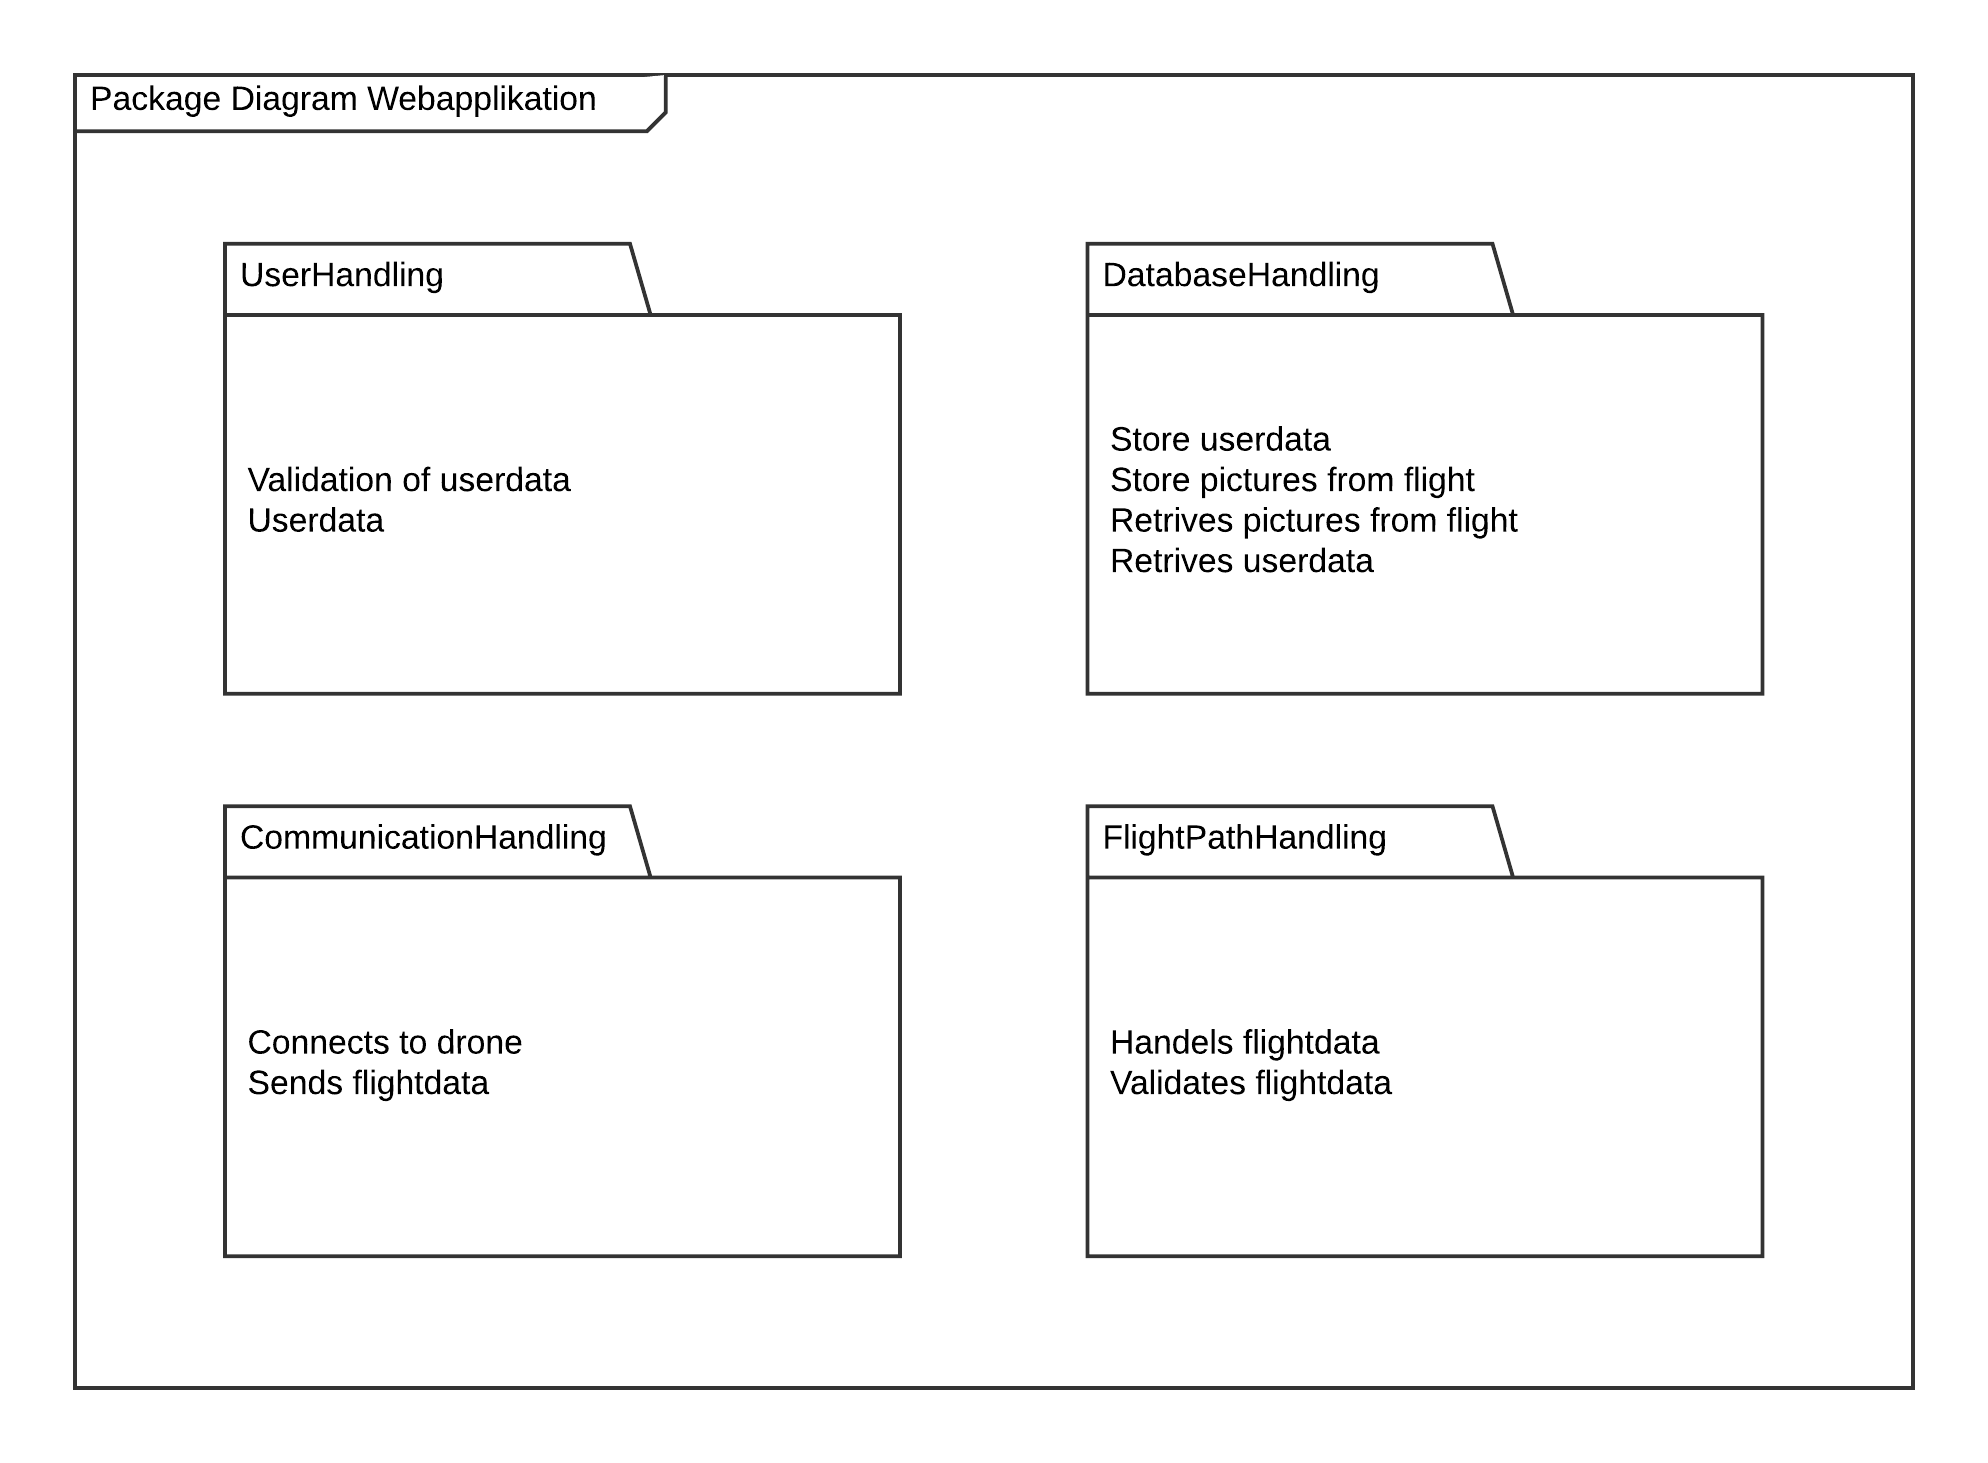
\includegraphics[width=1\textwidth]{Billeder/pakke_diagrammer/Gammel_server.png}
	\vspace{-1cm}
	\caption{Overordnet pakke diagram over webapplikationen}
	\label{fig:pakke_diagram_webapp}
\end{figure}

\textbf{CommunicationHandling}\\
Pakkens ansvar er kommunikation imellem drone og server. Pakken sender flyveinformation til dronen, som bruger har lavet på webapplikationen.

\textbf{UserHandling}\\
Pakkens ansvar er validering af login/log ud på websitet. Pakken har også ansvaret for at hente og gemme data om den pågældende bruger.

\textbf{DatabaseHandling}\\
Pakkens ansvar er kommunikation imellem databasen og serveren. 

\textbf{FlightPathHandling}\\
Pakkens ansvar er håndtering af flyveinformation samt validering af dataen.




\newpage
\subsection{Drone}

Figur \ref{fig:pakke_diagram_drone} viser pakkediagram over drone. 

\vspace{-5pt}
\begin{figure}[H]
	\centering
	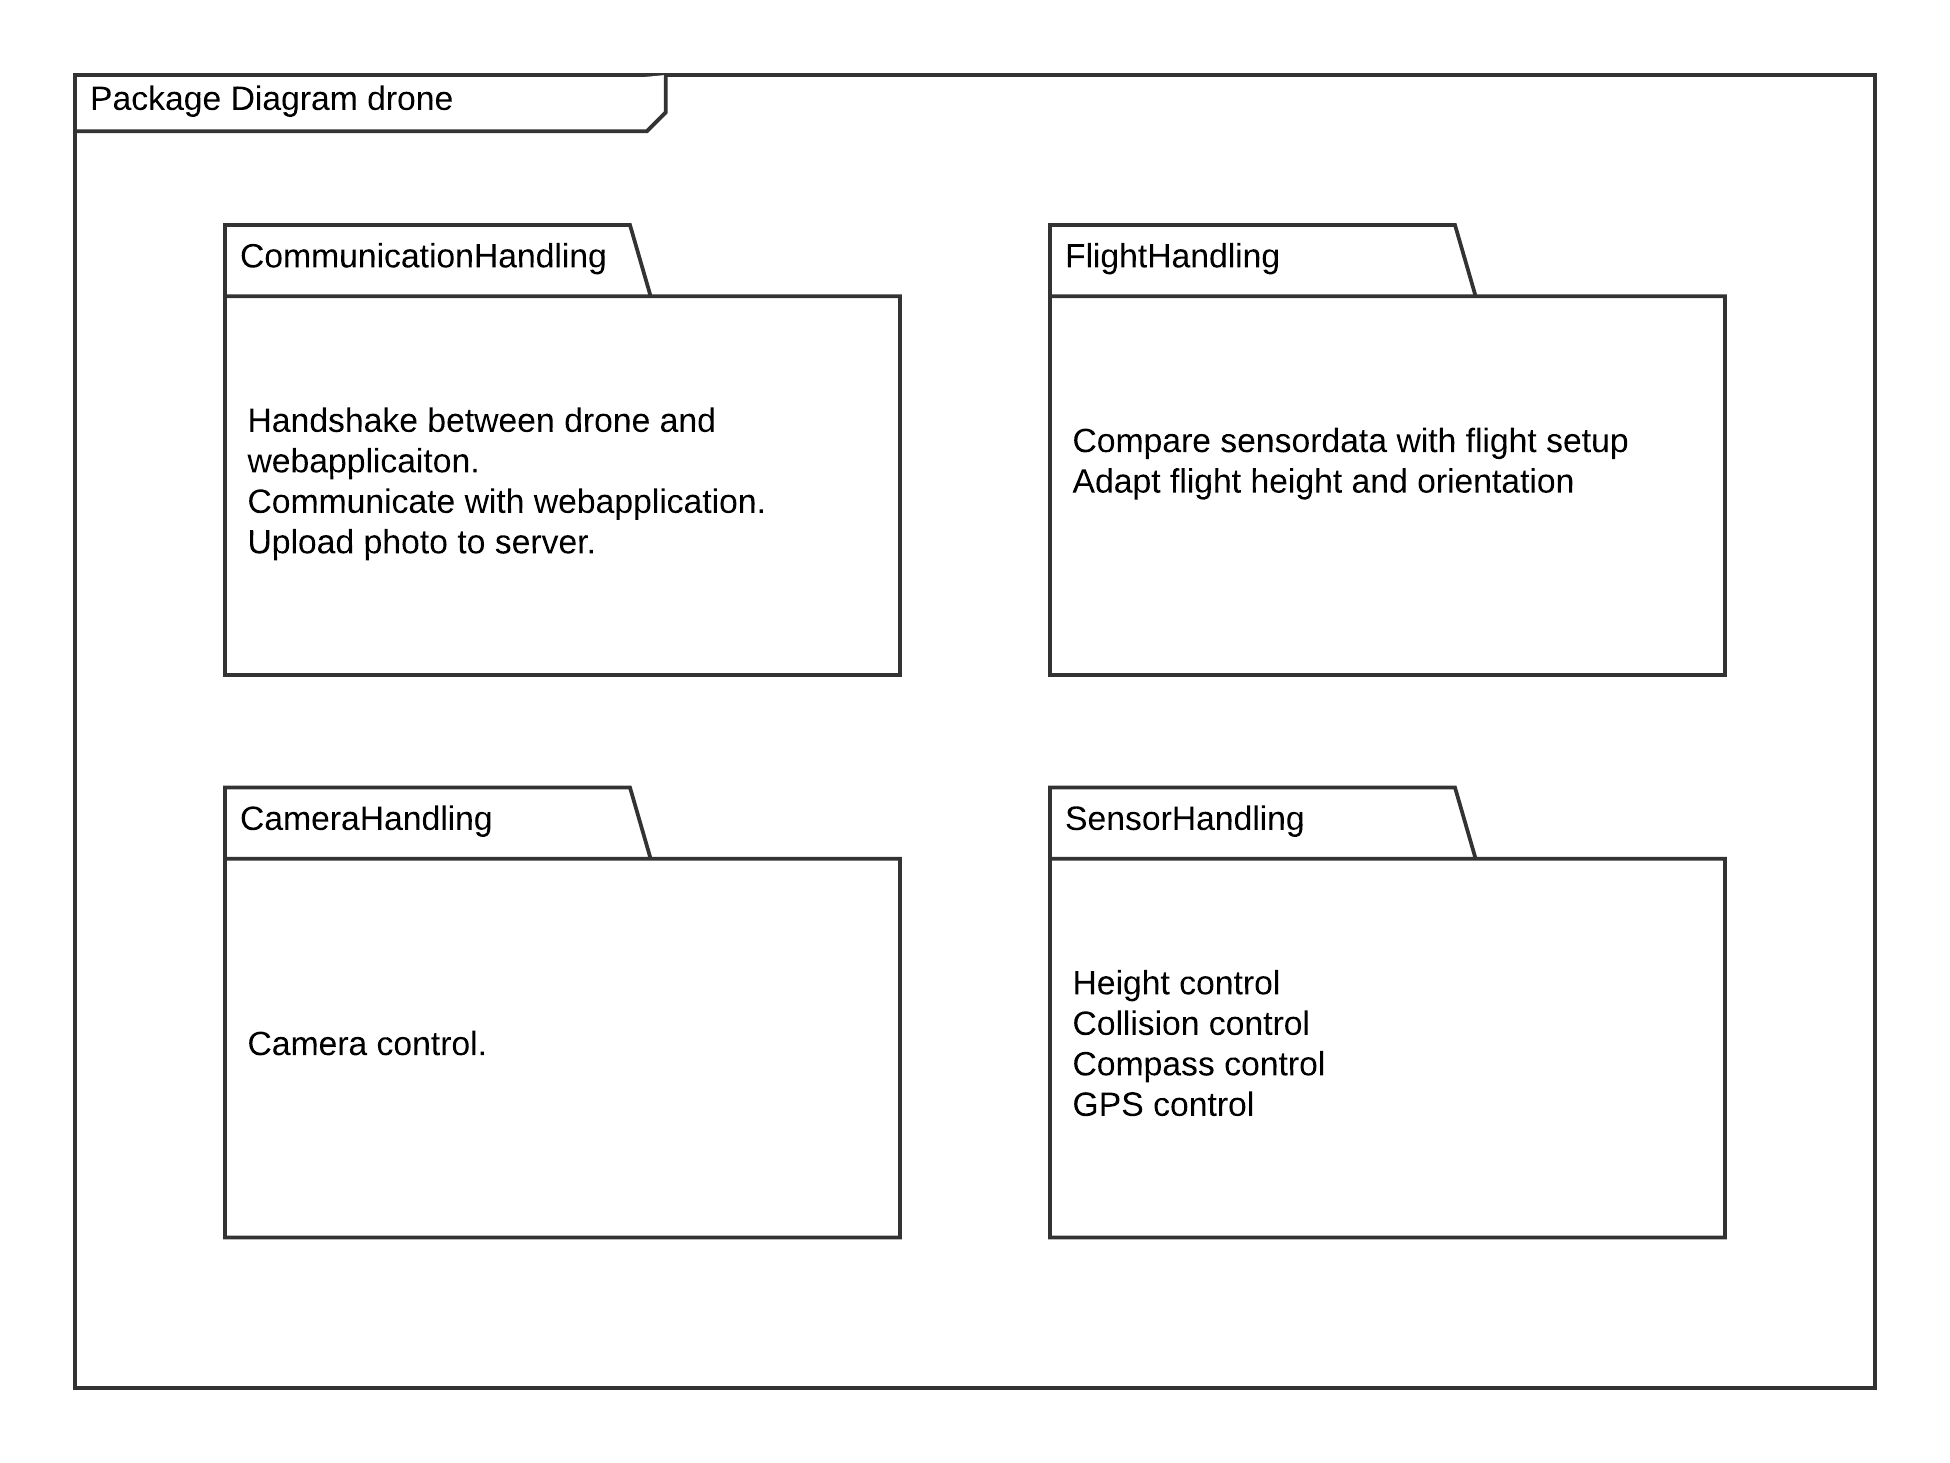
\includegraphics[width=1\textwidth]{Billeder/pakke_diagrammer/Gammel_drone.png}
	\vspace{-1cm}
	\caption{Overordnet pakke diagram over webapplikationen}
	\label{fig:pakke_diagram_drone}
\end{figure}

\textbf{CommunicationHandling}\\
Pakkens ansvar er kommunikation imellem drone og server. Pakken modtager flyveopsætning som bruger har lavet på webapplikationen og sender billeder til webapplikation.

\textbf{FlightHandling}\\
Pakkens ansvar er at sikre dronen flyver som angivet i flyveopsætning. Pakken har til ansvar at sammenligne data fra sensorer med den modtagne flyveopsætning, og ud fra det regulere dronens flyvehøjde og orientering. 

\textbf{CameraHandling}\\
Pakkens ansvar er håndtering af kamera. Der skal kun tages billeder med kameraet når dronen er på den rette GPS position. 

\textbf{SensorHandling}\\
Pakkens ansvar er håndtering af sensor data.
